\documentclass[11pt,a4paper]{article}

\title{F79MA: Assessed Project 2}
\author{Amit Parekh | H00184445}
\date{Semester 1, 2017}


% \usepackage{natbib}

\usepackage{amsmath}
\usepackage{amssymb}  % amssymb package contains more mathematical symbols
\usepackage{amsthm}  % asmthm package contains more theorem options

\usepackage{graphicx}  % graphicx package enables you to paste graphics into your document
\usepackage{color}  % color package adds ability to add colour

% \usepackage[letterspace=100]{microtype}  % Allows customising of letter spacing

\usepackage{mathtools}

\usepackage{fontspec}
\setmonofont[Contextuals={Alternate}]{FiraCode-Retina.otf}

\usepackage{listings}  % listings package allows better code presenting
    \lstloadlanguages{R}
    \lstdefinelanguage{Renhanced}[]{R}{%
      morekeywords={acf,ar,arima,arima.sim,colMeans,colSums,is.na,is.null,%
        mapply,ms,na.rm,nlmin,replicate,row.names,rowMeans,rowSums,seasonal,%
        sys.time,system.time,ts.plot,which.max,which.min,install.packages,\%>\%,\^ },
      deletekeywords={},
      alsoletter={.\%},%
      alsoletter={\%>\%},
      alsoother={:_\$}}
    \lstset{
        language=Renhanced,extendedchars=true, % Set language to R
        basicstyle=\ttfamily\scriptsize, % Monospaced font, small size (\footnotesize for smaller)
        keywordstyle=\color{ared}, % Commands as red
        commentstyle=\color{agreen}, % Comments as green
        % identifierstyle=\color{aorange}, % Variables as orange
        showstringspaces=false, % Remove spaces within strings
        escapeinside={@'}{@}, % Escape code mode
        delim=[is][\lsstyle]{@'}{@} % Letter spacing global in code mode
        literate={<-}{{$\gets$}}1
        index=[1][keywords], 
        indexstyle=\indexfonction
        }
        
\definecolor{ared}{rgb}{0.804,0.361,0.361}
\definecolor{agreen}{rgb}{0.235,0.702,0.443}

\newcommand{\expl}[1]{ \tag*{\textit{#1}} }



\usepackage{geometry}
 \geometry{
 a4paper,
%  total={170mm,257mm},
 left=12.7mm,
 top=12.7mm,
 bottom=25mm,
 right=12.7mm
 }

    \pagestyle{empty}
    \topmargin -1 cm
    \headheight 0cm
    \headsep 0cm
    % \textheight 27.16 cm
    % \textwidth 18.46 cm
    % \oddsidemargin 0 cm
    % \evensidemargin 0 cm
    \parindent 0 pt   % This sets the indentation for new paragraphs. Set to 20 pt (say) if you want new paragraphs indented.
    \parskip\smallskipamount

 \renewcommand{\P}{\textbf{P}}
 \newcommand{\E}{\textbf{E}}
 \renewcommand{\a}{\alpha}
 \renewcommand{\b}{\beta}
 \renewcommand{\th}{\theta}
 
\newcommand\numberthis{\addtocounter{equation}{1}\tag{\theequation}}
    
\usepackage{bm}
    
\usepackage{textcomp}
\newcommand{\textapprox}{\raisebox{0.5ex}{\texttildelow}}
\newcommand{\tilden}{\; \char`~ \;}

\usepackage{array}
\usepackage{booktabs}
\usepackage{multirow}
%%%%%%%%%%%%%%%%%%%%%%%%%%%%%%%%

\begin{document}

\maketitle
\thispagestyle{empty}

\section{Introduction}

This report contains an analysis of whether or not the company holds an appropriate amount of capital in reserve to cover the possible claims from a given set of policies. 

The probability that the total claims over the next year exceeds a reserve amount of $£1M$ is $0.0538$, which means that there is approximately a 1 in 20 chance that the company will not be have sufficient funds to pay out its claims for the following year. In order for the company to ensure a 99\% certainty that it will have sufficient funds to cover the claims for the next year, it needs to have at least $£5.66M$ in reserves. 

These results have been simulated using Jeffreys prior, using data of the total claims made per year for the last 10 years. 

\section{Analysis}

\subsection{Identifying a prior}

Due to a lack of experience with the policies of this form, I've used Jeffreys prior as it is a non-informative prior distribution for $\th$, meaning it only expresses vague information about $\th$ whilst supporting a wide range of possible values. Since it is also a flat prior, it will also have little impact on the posterior density. 

Jeffreys prior is defined as $$ \pi_j(\th) \propto \sqrt{I(\th)}, $$ where $I(\th)$ is the information function defined as,
\begin{align*}
    I(\th) &= \E \bigg( \Big[\frac{\partial}{\partial\th} \log L(\th; \underline X) \Big]^2 \bigg) \\
           &= - \E \bigg( \frac{\partial^2}{\partial\th^2} \log L(\th; \underline X) \bigg)
\end{align*}

Since the total claim amount in any given year $i$, is $x_i \sim Pareto(x_m,\theta)$, where $x_m = £0.1M$ and $\theta$ is an unknown shape parameter. Therefore, the density of the sample data is $$ f(\underline x; \theta) = \frac{\theta x_m^\theta}{x_i^{\theta+1}}. $$ From this, the likelihood function can be used to find Jeffreys prior:
\begin{align*}
    L(\theta; \underline{X}) &= \prod_{i=1}^n f(x_i;\theta)\\
                             &= \prod_{i=1}^n \; \frac{\theta x_m^\theta}{x_i^{\theta+1}} = \frac{\theta^n x_m^{n\theta}}{[\, \prod_{i=1}^n x_i]^{(\theta+1)}} \\
    \log L(\th;\underline X) &= n\log\th + n\th\log(x_m) - (\th + 1)\sum_{i=1}^n\log(x_i) \\
    \frac{\partial}{\partial\th}\log L(\th;\underline X) &= \frac{n}{\th} + n\log(x_m) - \sum_{i=1}^n\log(x_i) \\
    \frac{\partial^2}{\partial\th^2}\log L(\th;\underline X) &= \frac{-n}{\th^2} \\
    \therefore I(\th) &= -\E \bigg( \frac{-n}{\th^2} \bigg) = \frac{n}{\th^2} \\
    \therefore \pi_j(\th) &\propto \sqrt{I(\th)} = \sqrt{ \frac{n}{\th^2} } \propto \frac{1}{\th} \\
    \therefore \pi_j(\th) &= \frac{1}{\th}
\end{align*}

\subsection{The posterior density}

The posterior density $ \pi(\th | \underline x) $ can be derived from the prior density and the likelihood function. 
\begin{align*}
    \pi(\th | \underline x) &\propto \pi(\th) \times L(\th; \underline x) \\
                            &\propto \frac{1}{\th} \times \prod_{i=1}^n \, \frac{\theta \, x_m^\theta}{x_i^{\theta+1}} \\
                            &= \frac{1}{\th} \times \frac{\th^n \, x_m^{n\th}}{\prod_{i=1}^n x_i^{\th+1} } \\
                            &= \theta^{n-1} \times x_m^{n\th} \times \Bigg[ \prod_{i=1}^n x_i \Bigg]^{-(\th+1)} \\
                            \shortintertext{Removing the proportionality constant,}
                            &\propto \theta^{n-1} \times x_m^{n\th} \times \Bigg[ \prod_{i=1}^n x_i \Bigg]^{-\th} \\
                            &= \th^{n-1} \times e^{(n\th)\log x_m} \times e^{-\th\sum_{i=1}^n \log x_i} \\
                            &= \th^{n-1} \times e^{-\th(\sum_{i=1}^n\log x_i - n\log x_m)} \\
                            &\Rightarrow \th|\underline x \sim \Gamma(\a, \b), \text{ where } \a = n \text{, and } \b = \sum_{i=1}^n\log x_i - n\log x_m \\
                            &\Rightarrow \pi(\th|\underline{x}) = \frac{\b^\a}{\Gamma(\a)} \times \th^{\a-1} \times e^{-\b\th}
\end{align*}

\begin{figure}[!ht]
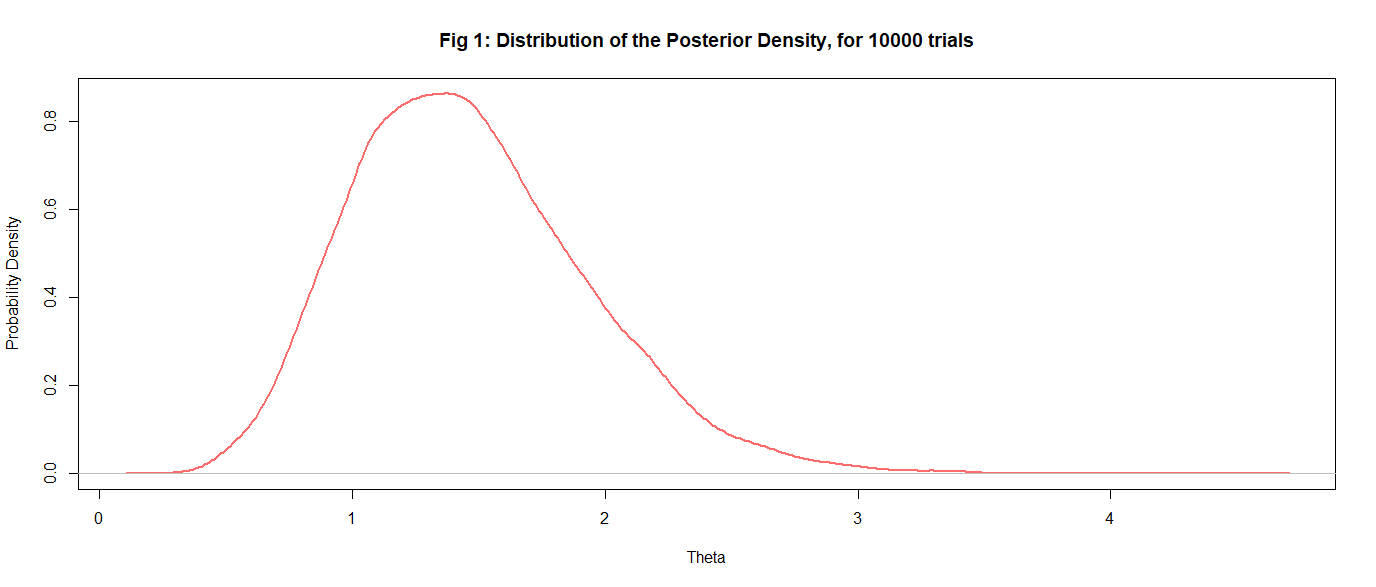
\includegraphics[width=\textwidth]{Q2_Graph_03.png}
\end{figure}
\begin{center}
{
    \setlength\extrarowheight{3pt}
    \noindent\begin{tabular}{|c c c c c c|}
        \hline
        \multicolumn{6}{|c|}{ \textbf{Table 1: 6-number summary of the posterior density} }\\
        \hline
        \textit{Minimum} & \textit{Lower Quartile} & \textit{Median} & \textit{Mean} & \textit{Upper Quartile} & \textit{Maximum} \\
        \hline
        0.3036 & 1.1242 & 1.4203 & 1.4674 & 1.7567 & 4.5033 \\
        \hline
    \end{tabular}
}
\end{center}

\subsection{Posterior predictive density}

Denote $y$ to be the total claim amount predicted for the next year. The predictive posterior density, $\pi(y|\underline x)$ can be derived from the posterior density and the marginal density of $y$. 

\begin{align*}
    \pi(y | \underline x) &= \int_0^\infty \pi(\th| \underline x) \times \pi(y|\th) \;\; d\th  \\
                          &= \int_0^\infty \frac{\b^\a}{\Gamma(\a)} \cdot \th^{\a-1} \cdot e^{-\b\th} \cdot \frac{\theta x_m^\theta}{y^{\theta+1}}  \;\;d\th\\
                          &= \frac{\b^\a}{\Gamma(\a)y} \int_0^\infty \th^{\a-1} \cdot e^{-\b\th} \cdot \frac{\theta x_m^\theta}{y^{\theta}} \;\;d\th \\ 
                          &= \frac{\b^\a}{\Gamma(\a)y} \int_0^\infty \th^{\a} \cdot e^{-\b\th} \cdot \Big( \frac{x_m}{y} \Big)^\th   \;\;d\th \\
                          &= \frac{\b^\a}{\Gamma(\a)y} \int_0^\infty \th^{\a} \cdot e^{-\b\th} \cdot e^{\th\log(\frac{x_m}{y})}  \;\; d\th  \\
                          &= \frac{\b^\a}{\Gamma(\a)y} \int_0^\infty \th^{\a} \cdot e^{ -\th(\b - \log(\frac{x_m}{y})) }   \;\;d\th \\
                          &= \frac{\b^\a}{\Gamma(\a)y} \int_0^\infty \th^{\a'-1} \cdot e^{-\th\b'} \;\;d\th, \\
                            \shortintertext{where $\a'=\a+1$, and $\b' = \b -\log(\frac{x_m}{y})$.}
            \Rightarrow \pi(y|\underline x) &= \frac{\b^\a}{\Gamma(\a)y} \int_0^\infty \th^{\a'-1} \cdot e^{-\th\b'} \cdot \frac{\Gamma(\a')}{\Gamma(\a')} \cdot \frac{\b'^{\a'}}{\b'^{\a'}} \;\;d\th \\ 
                          &= \frac{\b^\a}{\Gamma(\a)y} \int_0^\infty \underbrace{\frac{\b'^{\a'}}{\Gamma(\a')} \cdot \th^{\a'-1} \cdot e^{-\th\b'}}_\text{$=\Gamma(\a',\b')$} \cdot \frac{\Gamma(\a')}{\b'^{\a'}}\;\;d\th  \\
                          &= \frac{\b^\a \cdot \Gamma(\a')}{\Gamma(\a)y \cdot \b'^{\a'}} \underbrace{\int_0^\infty \Gamma(\a',\b')  \;\;d\th}_\text{$=1$} \\
                          &= \frac{\b^\a \cdot \Gamma(\a + 1)}{\Gamma(\a)y \cdot (\b-\log(\frac{x_m}{y}))^{\a+1}} \\
    \therefore \pi(y|\underline x) &= \frac{\a\b^\a}{y(\b-\log(\frac{x_m}{y}))^{\a+1}}
\end{align*}

\begin{figure}[!ht]
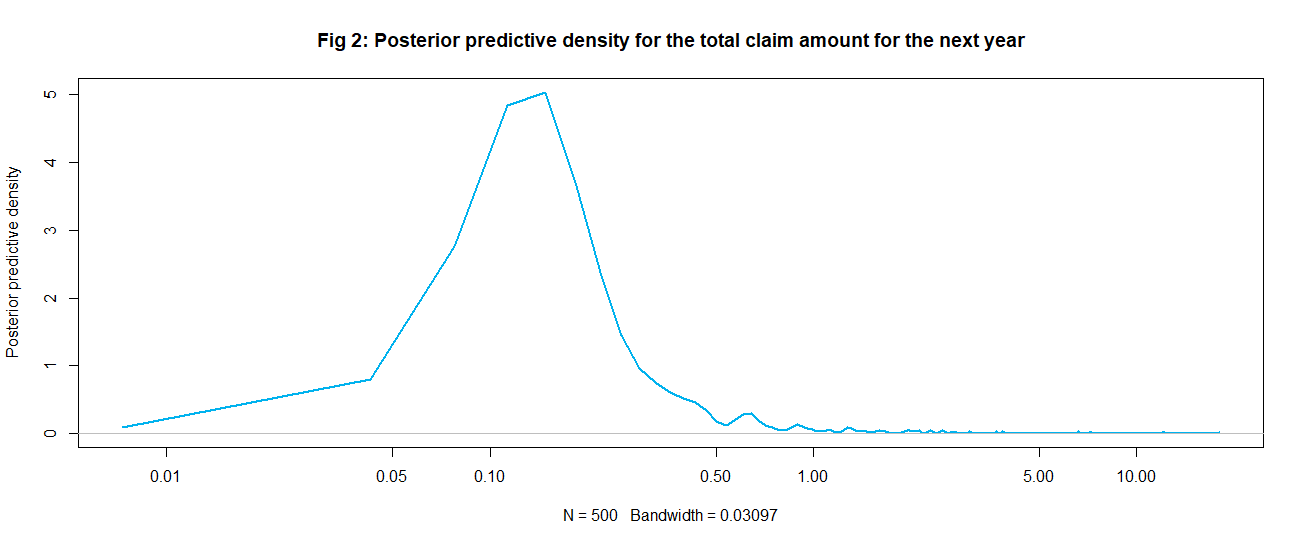
\includegraphics[width=\textwidth]{Q3_Graph_03.png}
\end{figure}
\begin{center}{
    \setlength\extrarowheight{3pt}
    \noindent\begin{tabular}{|c c c c c c|}
        \hline
        \multicolumn{6}{|c|}{ \textbf{Table 2: 6-number summary of the posterior predictive distribution} }\\
        \hline
        \textit{Minimum} & \textit{Lower Quartile} & \textit{Median} & \textit{Mean} & \textit{Upper Quartile} & \textit{Maximum} \\
        \hline
        0.1002 & 0.1190 & 0.1625 & 0.3924 & 0.2788 & 17.9433 \\
        \hline
    \end{tabular}
}
\end{center}

From simulating the Pareto distribution using the Inverse CDF technique,
\begin{align*}
    &\theta^{(i)} \sim \Gamma(\a,\b),\\
    &u^{(i)} \sim U[0,1], \\
    &\therefore y^{(i)} = \frac{x_m}{(1-u^{(i)})^{\frac{1}{\th}} } \\
    &\Rightarrow \P(Y > £1M), \text{ i.e. the expected number of }y^{(i)} \text{ that are greater than £1M}.
\end{align*}

The likelihood that the total claims next year exceeds the total reserve of $£1M$ is estimated to be $0.0538$, calculated from a simulation with a  suitably large sample size of $n=10000$. 


In order to ensure that the company is able to pay its claims for the following year with 99\% certainty, the company needs to have a reserve value of at least $£5.66M$. 

This is because, 
\begin{align*}
    \P(Y \leq reserve) = 0.99 \\
    \Rightarrow \P(Y > reserve ) = 0.01 \\
    \therefore reserve \geq £5.66M
\end{align*}

The Jeffreys posterior reflects the best possible information about $\th$ from the data, as the prior has little impact on the posterior. My advice is sensitive to the prior as it results in a posterior best reflecting the data available. If I were to change the prior, it could rely less on the previous 10 data points and could lead to different results entirely. 

\section{Appendix}

\subsection{Notes about code}
    Each section of code should be run independently of another. 
    
    I have use magrittr in the script, so if it doesn't work, check to see if the magrittr package is installed. You can run the code below to install and use magrittr prior to running a script.

    \begin{lstlisting}
    install.packages("magrittr")
    library("magrittr")
    \end{lstlisting}

\subsection{R code}

    \begin{lstlisting}
    # sample data
    x <- c(0.324, 0.177, 0.163, 0.317, 0.326, 0.174, 0.321, 0.115, 0.108, 0.133)
    n <- length(x)
    xMin <- 0.1
    
    # calculate beta
    b <- 0 
    for (i in 1:n) { b <- b + log(x[i]) }; b <- b - n*log(xMin)
    
    # calculate alpha
    a <- n 
    
    # Plot posterior density
    postDensity <- 0
    for (i in 1:10000) {
        postDensity[i] <- rgamma(1, a, b)
    }
    plot(density(postDensity),
         main = "Fig 1: Distribution of the Posterior Density, for 10000 trials",
         xlab="Theta", ylab="Probability Density",
         col="indianred1", lwd=2)
    summary(postDensity)
    
    # Simulate posterior predictive density
    y <- 0
    for (i in 1:500) {
        y[i] <- 0
        
        while (y[i] < 0.1) {
            u <- runif(1, 0, 1)
            theta <- rgamma(1, n, b)
            y[i] <- xMin / ( (1-u)^(1/theta) )
        }
    }
    plot(density(y), log="x", type='l',
        main = "Fig 2: Posterior predictive density for the total claim amount for the next year",
        ylab = "Posterior predictive density",
        col="deepskyblue2", lwd=2 )
    summary(y)
    
   # Estimate probability that y exceeds £1m
    y <- 0
    for (i in 1:10000) {
        y[i] <- 0
        while (y[i] < 0.1) {
            u <- runif(1, 0, 1)
            theta <- rgamma(1, n, b)
            y[i] <- xMin / ( (1-u)^(1/theta) )
        }
    }
    probest <- (y > 1) %>% sum() / 10000
    
    # Calculate reserve value
    reserve <- quantile(y, 0.99)
    probRes <- (y > reserve) %>% sum() / trials
    
    \end{lstlisting}

\end{document}